\documentclass[a4paper,graphics,11pt]{article}
\pagenumbering{arabic}

\usepackage[margin=1in]{geometry}
\usepackage[utf8]{inputenc}
\usepackage[T1]{fontenc}
\usepackage{lmodern}
\usepackage[ngerman]{babel}
\usepackage{amsmath, tabu}
\usepackage{amsthm}
\usepackage{amssymb}
\usepackage{complexity}
\usepackage{mathtools}
\usepackage{setspace}
\usepackage{graphicx,color,curves,epsf,float,rotating}
\usepackage{tasks}
\setlength{\parindent}{0em}
\setlength{\parskip}{1em}

\newcommand{\aufgabe}[1]{\subsection*{Aufgabe #1}}
\newcommand{\up}[2]{\mathrel{\overset{\makebox[0pt]{\mbox{\normalfont\tiny #2}}}{#1}}}
\newcommand{\re}{\operatorname{Re}}
\newcommand{\im}{\operatorname{Im}}

\begin{document}
\noindent Gruppe \fbox{\textbf{11}}             \hfill Tobias Riedel, 379133 \\
\noindent Analysis für Informatiker             \hfill Phil Pützstück, 377247 \\
\begin{center}
	\LARGE{\textbf{Hausaufgabe 8}}
\end{center}
\begin{center}
\rule[0.1ex]{\textwidth}{1pt}
\end{center}



\aufgabe{1}
\textbf{a)}\\[5pt]
Für $w_1$ gilt:
$$
    w_1 = \frac{2}{1-3i}
    = (2+0i)\cdot (1-3i)^{-1}
    = (2+0i) \cdot \left(\frac{1+3i}{1^2+3^2}\right)
    = (2+0i) \cdot \left(\frac{1}{10} + \frac{3}{10}i\right)
    = \frac{1}{5} + \frac{3}{5}i
$$
Es folgt
$$
    \re(w_1) = \frac{1}{5} \quad \text{und}\quad \im(w_1) = \frac{3}{5}
$$

Für $w_2$ gilt:
$$
    w_2 = \frac{1}{i}
    = (1+0i)\cdot (0+i)^{-1}
    = (1+0i)\cdot\left(\frac{0-i}{1}\right)
    = 0-i
$$
Es folgt
$$
    \re(w_2) = 0 \quad \text{und}\quad \im(w_2) = -1
$$

Für $w_3$ gilt:
$$
    w_3 = \frac{1+it}{1-it}
$$
Es folgt
$$
    \re(w_3) = \quad \text{und}\quad \im(w_3) = 
$$

\textbf{b)}
Nach Satz 1.6 lässt sich der Betrag $|z|$ wie folgt berechnen:
$$
    \left|\frac{(3+4i)(-1+2i)}{(-1-i)(3-i)}\right|
    = \frac{|(3+4i)(-1+2i)|}{|(-1-i)(3-i)|}
    =\frac{|3+4i|\cdot|-1+2i|}{|-1-i|\cdot|3-i|} 
    = \frac{5\cdot\sqrt{5}}{\sqrt{2}\cdot\sqrt{10}} = \frac{5}{2}
$$

\textbf{c)}
Sei $x,y \in \mathbb{R}$ mit $z=x+iy$. Es gilt
$$
    \left|\frac{z+i}{z-i}\right|
    = \frac{|z+i|}{|z-i|}
    = \frac{|(x+iy)+i|}{|(x+iy)-i|}
    = \frac{|x+i(y+1)|}{|x+i(y-1)|}
    = \sqrt{\frac{x^2+(y+1)^2}{x^2+(y-1)^2}}
    \leq 1
$$
Die lässt sich weiter umformen:
$$
    \sqrt{\frac{x^2+(y+1)^2 }{x^2+(y-1)^2}} \leq 1
    \,\Longleftrightarrow\, \frac{x^2+(y+1)^2}{x^2+(y-1)^2} \leq 1^2 = 1
    \,\Longleftrightarrow\, x^2+(y+1)^2 \leq x^2+(y-1)^2
$$$$
    \,\Longleftrightarrow\, (y^2+2y+1)-(y^2-2y+1) \leq 0
    \,\Longleftrightarrow\, 4y \leq 0
    \,\Longleftrightarrow\, y \leq 0
$$
Also ist die Ungleichung für alle $z \in \mathbb{C}$ mit $\im(z) \leq 0$ erfüllt.

\newpage

\textbf{d)}

\aufgabe{2}

\textbf{a)}
Mit $|z| = \sqrt{\re(z)^2+\im(z)^2}$ folgt
\begin{center}
    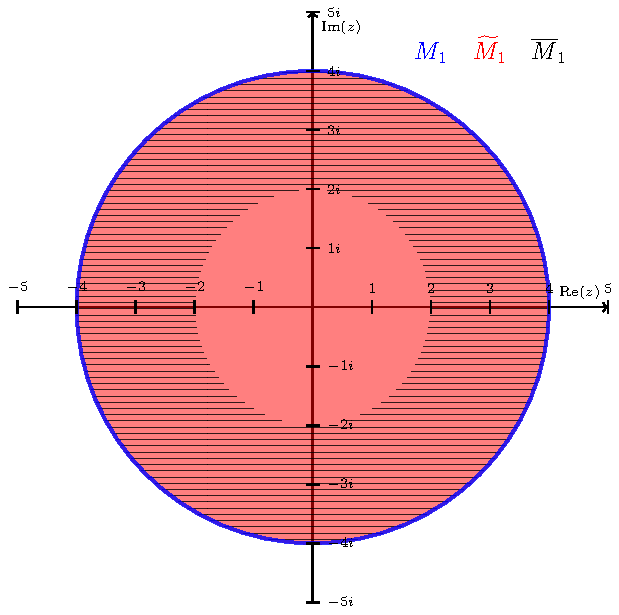
\includegraphics{graphics/graph1.pdf}
\end{center}
\textbf{b)}
Dies lässt sich wie eine Grade darstellen, welche $\im(z)$ in Relation zu $\re(z)$ setzt:
$$
    2\re(z) + 5\im(y) = 1
    \,\Longleftrightarrow\, \im(z) = \frac{1-2\re(z)}{5}
$$
\qquad\qquad\qquad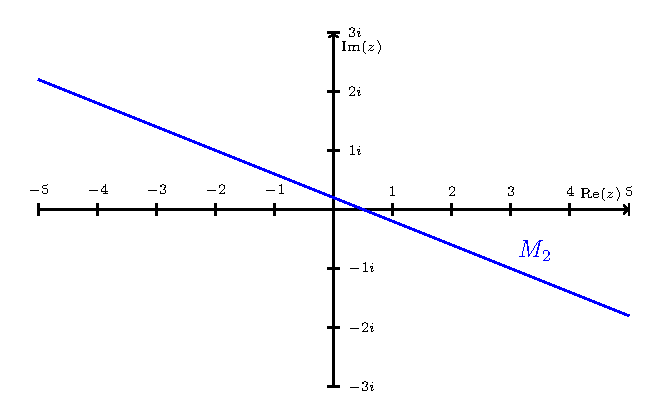
\includegraphics{graphics/graph2.pdf}
\newpage
\textbf{c)}
$$
    \re(z) + \im(z) -1 > 2
    \,\Longleftrightarrow\, \im(z) > 3-\re(z)
$$
Damit haben wir eine Geradengleichung. Alle werte ''über'' dieser gerade gehören zu $M_3$:\\
\strut\qquad\qquad\qquad\qquad\quad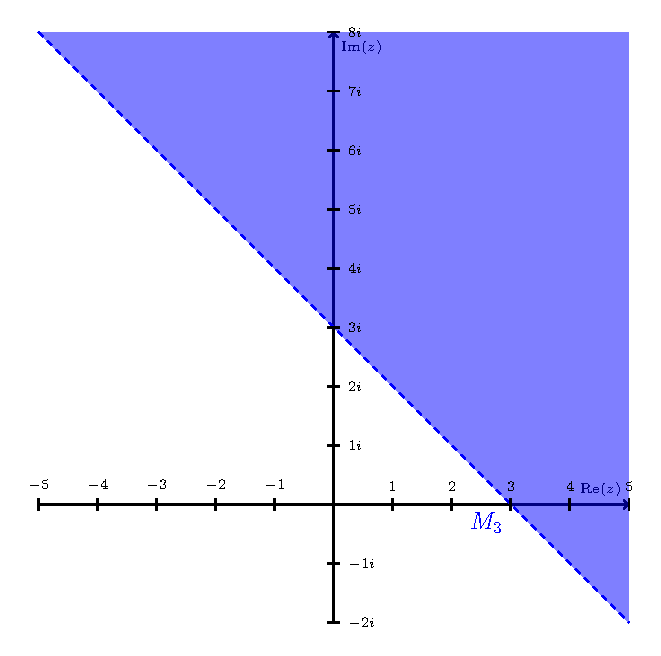
\includegraphics[scale=0.86]{graphics/graph3.pdf}

\textbf{d)}
Aus $\re(z) \geq 0$ folgt, dass alle Elemente von $M_4$ schonmal im 1. Quadranten liegen
müssen. Weiterhin muss $\im(z) \geq \re(z)$ gelten, also liegen alle Elemente von $M_4$
überhalb und auf der Geradengleichung $\im(z) = \re(z)$. Als letztes muss $|z| < 9$ gelten
wordurch das ganze mit dem Radius 9 beschränkt wird, daher das runde Ende:\\
\strut\qquad\qquad\qquad\qquad\quad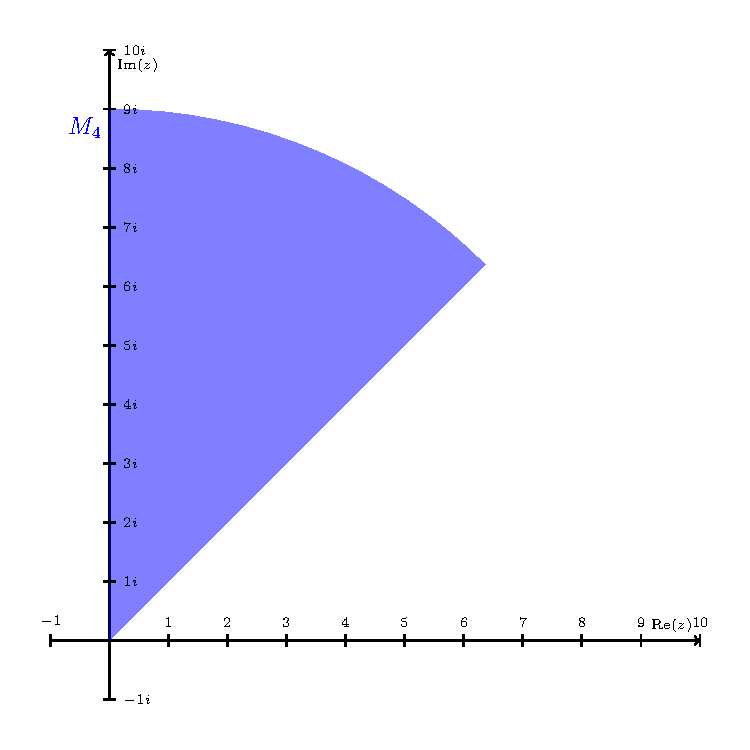
\includegraphics[scale=0.86]{graphics/graph4.pdf}
\newpage
\aufgabe{3}
Wir definieren:
\begin{align*}
    &(b_n)_{n\in \mathbb{N}} := 5i^{4n}\left(1+\frac{1}{n^3}\right)&
    (c_n)_{n\in \mathbb{N}} := 5i^{4n+1}\left(1+\frac{1}{n^3}\right)\\
    &(d_n)_{n\in \mathbb{N}} := 5i^{4n+2}\left(1+\frac{1}{n^3}\right) &
    (e_n)_{n\in \mathbb{N}} := 5i^{4n+3}\left(1+\frac{1}{n^3}\right)
\end{align*}
Es gilt
$$
    \forall n \in \mathbb{N}\colon i^{4n} = (i^2\cdot i^2)^n = ((-1)(-1))^n = 1^n = 1\\
$$
Es folgt
\begin{align*}
    \forall n \in \mathbb{N}\colon i^{4n+1} = i^{4n} \cdot i = i\\
    \forall n \in \mathbb{N}\colon i^{4n+2} = i^{4n} \cdot i^2 = i^2 = -1\\
    \forall n \in \mathbb{N}\colon i^{4n+3} = i^{4n} \cdot i^3 = i^3 = -i
\end{align*}
Weiterhin seien:
\begin{align*}
    &(w_n)_{n\in \mathbb{N}} := 4n&
    (x_n)_{n\in \mathbb{N}} := 4n+1\\
    &(y_n)_{n\in \mathbb{N}} := 4n+2&
    (z_n)_{n\in \mathbb{N}} := 4n+3
\end{align*}
Dann gilt für alle $n\in \mathbb{N}$ stets:
\begin{align*}
    &b_n = \left(1+\frac{1}{n^3}\right)=  5i^{4n}\left(1+\frac{1}{n^3}\right) = a_{w_n}&
    c_n = i\cdot\left(1+\frac{1}{n^3}\right)5i^{4n+1}\left(1+\frac{1}{n^3}\right) = a_{x_n}\\
    &d_n = -\left(1+\frac{1}{n^3}\right) = 5i^{4n+2}\left(1+\frac{1}{n^3}\right) = a_{y_n}&
    e_n = -i\cdot\left(1+\frac{1}{n^3}\right)=5i^{4n+3}\left(1+\frac{1}{n^3}\right) = a_{z_n}
\end{align*}
Folglich sind $b_n,c_n,d_n$ und $e_n$ alle Teilfolgen von $a_n$.
Die Grenzwertsätze lassen sich wie folgt anwenden:
$$
    \lim_{n \to \infty} b_n
    = \lim_{n \to \infty} 1+ \lim_{n \to \infty} \frac{1}{n^3}
    = 1+0 =1\\
$$$$
    \lim_{n \to \infty} c_n
    = \lim_{n \to \infty} i+ \lim_{n \to \infty} i\cdot \frac{1}{n^3}
    = i+\lim_{n \to \infty} i\cdot \lim_{n \to \infty} \frac{1}{n^3}
    = i+i\cdot 0 = i
$$$$
    \lim_{n \to \infty} d_n
    = \lim_{n \to \infty} -1 - \lim_{n \to \infty} \frac{1}{n^3}
    = -1 - 0 = -1
$$$$
   \lim_{n \to \infty} e_n
    = \lim_{n \to \infty} -i- \lim_{n \to \infty} i\cdot \frac{1}{n^3}
    = -i-\lim_{n \to \infty} i\cdot \lim_{n \to \infty} \frac{1}{n^3}
    = -i-i\cdot 0 = -i
$$
Also folgt für die Teilfolgen $b_n,c_n,d_n,e_n$ von $a_n\colon$
$$
    \lim_{n \to \infty} b_n \neq
    \lim_{n \to \infty} c_n \neq
    \lim_{n \to \infty} d_n \neq
    \lim_{n \to \infty} e_n
$$
\newpage
\aufgabe{4}




\end{document}
